\documentclass[a4paper]{article}
\usepackage{amssymb}
\usepackage{array}
\usepackage{amsmath}
\usepackage[affil-it]{authblk}
\usepackage[backend=bibtex,style=numeric]{biblatex}
\usepackage{graphicx}
\usepackage{geometry}
\usepackage{subfig}
\geometry{margin=1.5cm, vmargin={0pt,1cm}}
\setlength{\topmargin}{-1cm}
\setlength{\paperheight}{29.7cm}
\setlength{\textheight}{25.3cm}

\addbibresource{citation.bib}

\begin{document}
% =================================================
\title{Numerical Analysis homework \# 4}

\author{Chen Shuo 12231064
  \thanks{Email address: \texttt{shuo\_chen@zju.edu.cn}}}
\affil{(Electronic Science and Technology), Zhejiang University }


\date{Submitted time: \today}

\maketitle
% ============================================
\section*{I}
$477 = (111011101)_2=(1.1101101)_2\times 2^7$
\section*{II}
$\frac{3}{5} = (0.\overline{1001})_2 = (1.\overline{0011})_2\times 2^{-1}$
\section*{III}
$$
x = \beta^e = 1\times \beta^e \Longrightarrow x_R = 2\times \beta^e, x_R - x = \beta^e
$$
$$
x = \beta^e = \beta\times \beta^{e-1} \Longrightarrow x_L = (\beta-1)\times \beta^{e-1}, x - x_L = \beta^{e-1}
$$
$$
\therefore x_R - x = \beta(x - x_L)
$$
\section*{IV}
According to the result of II, $\dfrac{3}{5} = (1.\overline{0011})_2\times 2^{-1}$. In IEEE 754 single-precision protocal, 
there are 23 bits for the significand, so:
$$
\frac{3}{5} = (1.0011001\cdots)_2 \times 2^{-1}
$$
$$
x_L = (1.0011001\cdots001)_2 \times 2^{-1}
$$
$$
x_R = (1.0011001\cdots010)_2 \times 2^{-1}
$$
$$
x - x_L = \frac{3}{5} \times 2^{-24}
$$
$$
x_R - x = \frac{2}{5} \times 2^{-24}
$$
Therefore $\text{fl}(x) = x_R$, roundoff error is $|\text{fl}(x) - x| = \dfrac{2}{5} \times 2^{-24}$.

\section*{V}
If the excess bits are simply dropped, then the $(0,1)\times2^{-23}$ part would be eliminated. The unit roundoff is $\sup((0,1) \times 2^{-23}) = 2^{-23}$.

\section*{VI}
According to Theorem 4.49, $\beta^{-t}\leq 1 - \dfrac{y}{x} \leq \beta{-s}$. In this case, $\beta = 2$, $y = \cos{\dfrac{1}{4}}$, $x=1$. And $1-\cos{\dfrac{1}{4}} \approx 0.0311$, $2^{-5}\leq0.0311\leq2^{-4}$.
Therefore it would lose 4 or 5 bits of precision.

\section*{VII}
\begin{itemize}
  \item By using Taylor series: $1-\cos{x}=1-(1-\dfrac{x^2}{2}+\dfrac{x^4}{4}-\dfrac{x^6}{6}+\cdots)=\dfrac{x^2}{2}-\dfrac{x^4}{4}+\dfrac{x^6}{6}+\cdots$
  \item $1-\cos{x} = \dfrac{(1-\cos{x})(1+\cos{x})}{1+\cos{x}} = \dfrac{1-\cos^2{x}}{1+\cos{x}} = \dfrac{\sin^2{x}}{1+\cos{x}}$
\end{itemize}

\section*{VIII}
According to the definition, $C_{f}(x) = |\dfrac{xf'(x)}{f(x)}|$.
\begin{itemize}
  \item $f(x) = (x-1)^\alpha$, $f'(x) = \alpha(x-1)^{\alpha-1}$, $C_{f}(x) = |\dfrac{\alpha x}{x-1}|$, $C_{f}(x)$ are large when $x \rightarrow 1$.
  \item $f(x) = \ln x$, $f'(x) = \dfrac{1}{x}$, $C_{f}(x) = |\dfrac{1}{\ln x}|$, $C_{f}(x)$ are large when $x \rightarrow 1$.
  \item $f(x) = e^x$, $f'(x) = e^x$, $C_{f}(x) = |x|$, $C_{f}(x)$ is large when $|x|$ is large.
  \item $f(x) = \arccos x$, $f'(x) = -\dfrac{1}{\sqrt{1-x^2}}$, $C_{f}(x) = |\dfrac{x}{\sqrt{1-x^2}\arccos x}|$, $C_{f}(x)$ are large when $x \rightarrow \pm 1$ or $x \rightarrow \dfrac{\pi}{2}$.
\end{itemize}
\section*{IX}
\subsection*{IX-a}
$$
\text{cond}_f(x) = |\frac{xf'(x)}{f(x)}| = \frac{xe^{-x}}{1-e^{-x}}, x \in (0,1]
$$
$$
\text{cond}_f(0) = \lim_{x\rightarrow0^{+}}|\frac{xe^{-x}}{1-e^{-x}}| = 1
$$
We have $\dfrac{xe^{-x}}{1-e^{-x}} = \dfrac{x}{e^x-1}$ and $g(x) < 1$ since $0 < x < e^x -1$, so $\text{cond}_f(x) \leq 1$ for $x \in [0,1]$.

\subsection*{IX-b}
Apply Theorem 4.78 to analyze the conditioning of the algorithm:
$$
f_A = \text{fl}(1-\text{fl}(e^{-x}))
$$
By neglecting the quadratic terms of $O(\delta_i^2)$:
$$
f_A(x) = (1-e^{-x}(1+\delta_1))(1+\delta_2) = (1-e^{-x})(1+\delta_2-\frac{e^{-x}}{1-e^{-x}}\delta_1),
$$
where $|\delta_i| \leq \epsilon_u$ for $i = 1,2$. Hence we have $\phi(x) = 1 + \dfrac{e^{-x}}{1-e^{-x}} = \dfrac{1}{1-e^{-x}}$ and
$$
\text{cond}_A(x) \leq \frac{1-e^{-x}}{xe^{-x}}\cdot\dfrac{1}{1-e^{-x}} = \frac{e^x}{x}
$$
\section*{IX-c}
$\text{cond}_f(x)$ is plotted as Figure 1.
\begin{figure}[htbp]
  \centering
  \subfloat[$\text{cond}_f(x)$]{
    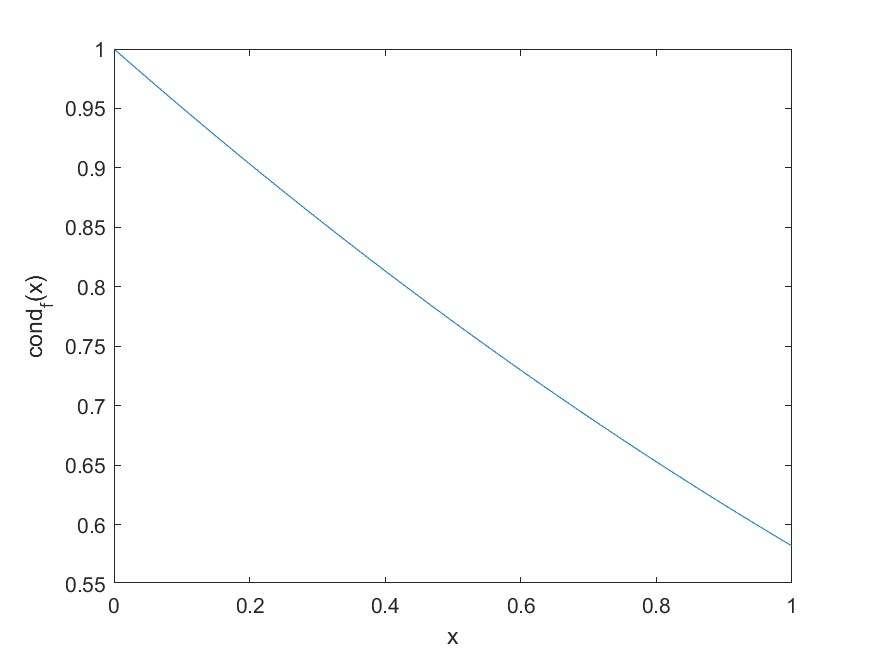
\includegraphics[width=0.5\textwidth]{fig/ProblemIX-c1.jpg}
  }
  \subfloat[estimated upper bound of $\text{cond}_A(x)$]{
    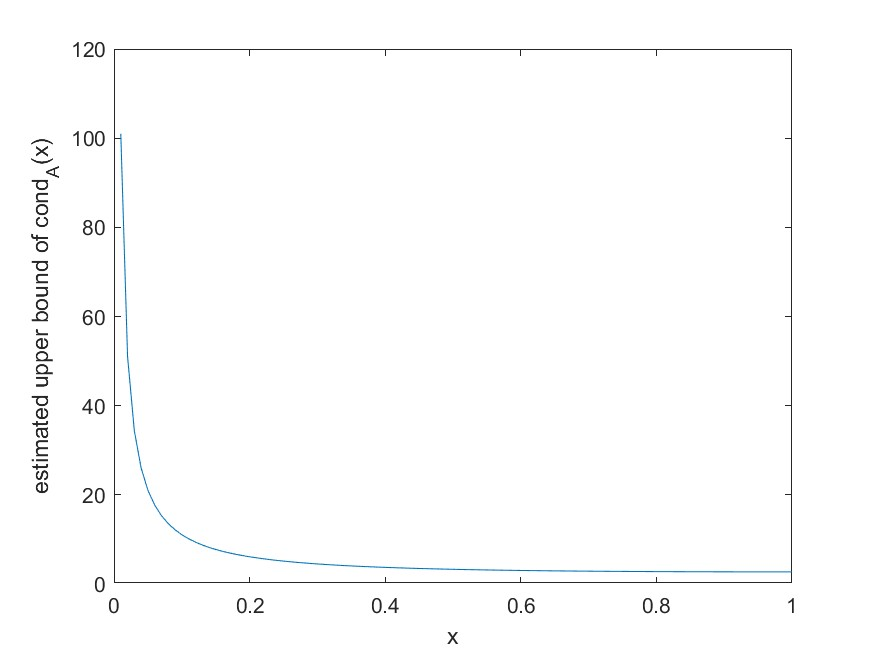
\includegraphics[width=0.5\textwidth]{fig/ProblemIX-c2.jpg}
  }
  \caption{ProblemIX}
\end{figure}

By IX-b, $\text{cond}_A(x)$ may be unbounded at $x = 0$. On the other hand, $\text{cond}_A(x)$ is controlled by $e$ as $x\rightarrow\frac{\pi}{2}$.

\section*{X}
Do SVD to $A$, i.e. $A = U\Sigma V^T$, $U$, $V$ are orthogonal matrices and $\Sigma = \text{diag}\{\sigma_1,\cdots\sigma_m\}$, $\sigma_i$ is the singular value of $A$ with $\sigma_1 \geq \sigma_2 \geq \cdots \geq \sigma_m > 0$.
According to the definition of 2-norm:
$$
||A||_2 = \sup\limits_{x}\frac{||Ax||_2}{||x||_2} = \sup\limits_{||x||_2=1}||Ax||_2=\sup\limits_{||x||_2=1}||\Sigma x||_2
= \sup\limits_{||x||_2=1}\sqrt{\sigma_1^2 x_1^2 + \cdots + \sigma_m^2 x_m^2} = \sigma_1 = \sigma_{max}
$$
$A^{-1} = V\Sigma^{-1}U^T$, and $\Sigma^{-1} = \text{diag}\{\sigma^{-1},\cdots\sigma_m^{-1}\}$. Similarly we can get $||A^{-1}||_2 = \sigma_m^{-1} = \sigma_{min}^{-1}$.

Therefore, $\text{cond}_2 A = ||A||_2 ||A^{-1}||_2 = \dfrac{\sigma_{max}}{\sigma_{min}}$.

If $A$ is normal, then $\{\sigma_i\}$ of $\Sigma$ in SVD are the norm of eigenvalues of $A$, so $\text{cond}_2 A = \dfrac{|\lambda|_{max}}{|\lambda|_{min}}$.

\section*{XI}
$$
\sum\limits_{j=0}^n a_j r^j = 0
$$
Consider $r$ as the function of $a_j$ and take derivates with $a_j$ for two sides:

If $j \neq 0$,
$$
r^j + a_j j r^{j-1} \frac{\partial r}{\partial a_j} + \sum\limits_{k=1,k\neq j}^n a_k k r^{k-1} \frac{\partial r}{\partial a_j}
= r^j + \sum\limits_{k=1}^n a_k k r^{k-1} \frac{\partial r}{\partial a_j} = 0
\Longrightarrow
\frac{\partial r}{\partial a_j} = -\frac{r^j}{\sum\limits_{k=1}^n a_k k r^{k-1}}
$$

If $j = 0$,
$$
1 + \sum\limits_{k=1}^n a_k k r^{k-1} = 0
\Longrightarrow
\frac{\partial r}{\partial a_j} = -\frac{1}{\sum\limits_{k=1}^n a_k k r^{k-1}}
$$
Therefore 2 cases can be conbimed into 1, i.e. $\dfrac{\partial r}{\partial a_j} = -\dfrac{r^j}{\sum\limits_{k=1}^n a_k k r^{k-1}}$, $j = 0,1,\cdots,n-1$.

Let $\textbf{y} = (a_0,\cdots,a_{n-1})$ and according to Definition 4.71, $\text{cond}_f(\textbf{y}) = ||A(\textbf{y})||$. In this case $A(\textbf{y}) \in \mathbb{R}^{1\times n}$, 
$a_{1j}(\textbf{y}) = \Bigg| \dfrac{y_j\frac{\partial f}{\partial y_j}}{f(\textbf{y})} \Bigg|
= \dfrac{|a_{j-1}r^{j-1}|}{|\sum\limits_{k=1}^n a_k k r^k|}$. Here we use 1-norm and $\text{cond}_f(\textbf{y}) = ||A(\textbf{y})||_1 = \sum\limits_{j=1}^{n}|a_{1j}| = \dfrac{\sum\limits_{k=0}^{n-1}|a_k r^k|}{|\sum\limits_{k=1}^n a_k k r^k|}$

For the Wilkinson example, $r = 1,2,\cdots,p$. Let $h(x) = \prod\limits_{k=1}^p (x+k)$, and $\sum\limits_{k=0}^{n-1}|a_k r^k| = h(r)$. The denominator term $|\sum\limits_{k=1}^n a_k k r^k| = |f'(r)| = |\sum\limits_{j=1}^p\prod\limits_
{k=1,k\neq j}^p (r-k)|$. Let $r = m \in \{1,2,\cdots,p\}$, $\text{cond}_f(\textbf{y}) = \dfrac{h(r)}{|f'(r)|} = \dfrac{m(m+1)\cdots(m+p)}{\prod\limits_{k=1,k\neq j}^p(r-k)} = \dfrac{(m+p)!}{m!(m-1)!(p-m)!}$. For the root $r = p$, 
$\text{cond}_f(\textbf{y}) = \dfrac{(2p)!}{p!(p-1)!}$.

For p = 20, 30, 40, $\text{cond}_f(\textbf{y})$ is about $2.8\times 10^{12}, 3.5\times 10^{18}, 4.3\times 10^{24}$, respectively. Comparing the result with that in the Wilkinson Example, the problem of root finding for polynomials with very high degrees is hopeless.

\section*{XII}
By Definitions 4.24, 4.16, and 4.26, the unit roundoff of a register with precision $2p$ is
$$
\frac{1}{2}\beta^{1-2p} = \frac{1}{2} \beta^{1-p} \beta^{1-p} \beta^{-1} = \beta^{-1} \epsilon_u \epsilon_M
$$
Let $M_a = a = 1, M_b = b = \beta - \epsilon_M$, then:
$$
M_{c1} = \frac{M_a}{M_b} + \delta_1, |\delta_1| < \beta^{-1} \epsilon_u \epsilon_M
$$
$$
M_{c2} = \beta M_{c1} + \delta_2 = \beta \frac{M_a}{M_b}(1 + \frac{\beta\delta_1 + \delta_2}{\beta M_a/M_b}) = \beta \frac{M_a}{M_b}(1 + (\beta-\epsilon_M)\delta_1 + \frac{\beta - \epsilon_M}{\beta}\delta_2), |\delta_2| < \epsilon_u
$$
Let $\delta_1 = \beta^{-1} \epsilon_u \epsilon_M - \epsilon_1 < \beta^{-1} \epsilon_u \epsilon_M$, $\delta_2 = \epsilon_u - \epsilon_2 < \epsilon_u$. Choose $\epsilon_1 = \dfrac{\epsilon_u\epsilon_M^2}{\beta(\beta-\epsilon_M)}$, 
$\epsilon_2 = \dfrac{\epsilon_u\epsilon_M^2}{\beta-\epsilon_M}$, then:
\begin{align*}
  |\delta| &= |(\beta-\epsilon_M)\delta_1 + \frac{\beta - \epsilon_M}{\beta}\delta_2| \\
  &= \frac{(\beta - \epsilon_M)\epsilon_u\epsilon_M}{\beta} - \frac{\epsilon_u\epsilon_M^2}{\beta} + \frac{(\beta - \epsilon_M)\epsilon_u}{\beta} - \frac{\epsilon_u\epsilon_M^2}{\beta} \\
  &= \frac{\epsilon_u}{\beta}(\beta + (\beta - 1)\epsilon_M - 3\epsilon_M^2) \\
  &> \frac{\epsilon_u}{\beta}\cdot\beta
  = \epsilon_u
\end{align*}
The result contradicts the conclusion of the model of machine arithmetic, which says $|\delta| < \epsilon_u$.



\section*{XIII}
In single precision FPNs of IEEE 754, $[128,129]$ can be represented as $[1,1+\dfrac{1}{2^7}]\times 2^7$(not expanded into binary form for convenience). If we want the absolute accuracy of $10^{-6}$, i.e. $2^{-19}$ or $2^{-20}$, it means the significand should be 
$2^{-26}$ or $2^{-27}$, since the exponent part is $2^7$. But this exceed the bits of single precision, which is only 23.

Therefore we cannot compute the root with absolute accuracy $< 10^{-6}$.

\section*{Exercise 4.33}
\subsection*{a}
$a = 1.234 \times 10^4$, $b = 8.769 \times 10^4$

(i) do nothing.

(ii) $m_c \leftarrow 10.003$.

(iii) $m_c \leftarrow 1.0003$; $e_c \leftarrow 5$.

(iv) do nothing.

(v) $m_c \leftarrow 1.000$.

(vi) $c = 1.000 \times 10^5$.

\subsection*{b}
$a = 1.234 \times 10^4$, $b = -5.678 \times 10^0$

(i) $b \leftarrow -0.0005678 \times 10^4$; $e_c \leftarrow 4$.

(ii) $m_c \leftarrow 1.2334322$.

(iii) do nothing.

(iv) do nothing.

(v) $m_c \leftarrow 1.233$.

(vi) $c = 1.233 \times 10^4$.

\subsection*{c}
$a = 1.234 \times 10^4$, $b = -5.678 \times 10^3$

(i) $b \leftarrow -0.5678 \times 10^4$; $e_c \leftarrow 4$.

(ii) $m_c \leftarrow 0.7662$.

(iii) $m_c \leftarrow 7.662$; $e_c \leftarrow 3$.

(iv) do nothing.

(v) do nothing.

(vi) $c = 7.662 \times 10^3$.


\section*{Exercise 4.42}
Let $a_0 = 1, a_1 = 2, a_2 =3$.

(i) Add in the ascending order:
\begin{itemize}
  \item $s_1 = 3$, $s_2 = 6$,$\delta_1 = \epsilon_0$
  \item $\delta_2 = \epsilon_1 + \delta_1(1 + \epsilon_1)\dfrac{s_1}{s_2} = \epsilon_1 + \dfrac{\epsilon_0}{2}(1 + \epsilon_1)$
\end{itemize}

(ii) Add in the descending order:
\begin{itemize}
  \item $s_1 = 5$, $s_2 = 6$,$\delta_1 = \epsilon_0$
  \item $\delta_2 = \epsilon_1 + \delta_1(1 + \epsilon_1)\dfrac{s_1}{s_2} = \epsilon_1 + \dfrac{5\epsilon_0}{6}(1 + \epsilon_1)$
\end{itemize}
Compare 2 results and $\delta_2$ in case (i) is smaller.

\section*{Exercise 4.43}
By neglecting the terms of $O(\delta_i^2)$, we get:
\begin{align*}
  &\text{fl}(a_1 b_1 + a_2 b_2 + a_3 b_3) \\
  &= \text{fl}(\text{fl}(\text{fl}(a_1 b_1) + \text{fl}(a_2 b_2)) + \text{fl}(a_3 b_3)) \\
  &= ((a_1 b_1(1+\delta_1) + a_2 b_2(1+\delta_2))(1 + \delta_3) + a_3 b_3(1 + \delta_4))(1 + \delta_5) \\
  &= (a_1 b_1 + a_2 b_2 + a_3 b_3)\\
  &\cdot(1+\delta_5 + (\delta_1 + \delta_3)\frac{a_1 b_1}{a_1 b_1 + a_2 b_2 + a_3 b_3} + (\delta_2 + \delta_3)\frac{a_2 b_2}{a_1 b_1 + a_2 b_2 + a_3 b_3} + \delta_4\frac{a_3 b_3}{a_1 b_1 + a_2 b_2 + a_3 b_3}) \\
  &< (a_1 b_1 + a_2 b_2 + a_3 b_3)(1 + 3\epsilon_u)
\end{align*}
Guess that $\text{fl}(\sum_{i=1}^{m}\prod_{j=1}^{n}a_{i,j}) = (\sum_{i=1}^{m}\prod_{j=1}^{n}a_{i,j})(1 + (n-1)m\delta_n)$, where $|\delta_n| < \epsilon_u$.




\section*{Exercise 4.80}
Similar with Example 4.79:
$$
f_A = \text{fl}\Big[\frac{\text{fl}(\sin x)}{\text{fl}(1 + \text{fl}(\cos x))}\Big]
$$
$$
f_A(x) = \frac{\sin x(1 + \delta_3)}{(1 + \cos x(1 + \delta_1))(1 + \delta_2)}(1 + \delta_4)
$$
Neglecting the terms of $O(\delta_i^2)$, the above equation is equivalent to
$$
f_A(x) = \frac{\sin x}{1 + \cos x}(1 + \delta_3 + \delta_4 - \delta_2 - \delta_1\frac{\cos x}{1 + \cos x})
$$
Hence we have $\phi(x) = 3 + \frac{\cos x}{1 + \cos x}$ and
$$
\text{cond}_A(x) \leq \frac{\sin x}{x}(3 + \frac{\cos x}{1 + \cos x}).
$$
Obviously $\text{cond}_A(x)$ is bounded for $x \in (0,\pi/2)$.









\end{document}


